% BDC223 Lecture 7b: Measuring Photosynthesis. Summary slides with TikZ figures.
% Data plotted on slides come from models.py (data/*.dat); all are illustrative simulations.
\documentclass[aspectratio=169,11pt]{beamer}
\usepackage[sfdefault,lining]{FiraSans}
\usepackage{amsmath}
\usefonttheme{professionalfonts}
\usepackage{firamath-otf}
\setmathrm{Fira Sans}
\usepackage{tikz}
\usepackage{pgfplots}
\usepackage{booktabs}
\usepackage{array}
\pgfplotsset{compat=1.18,every axis/.append style={width=7.1cm}}
\usetikzlibrary{arrows.meta,calc,decorations.pathmorphing,shapes.geometric,positioning,patterns}

\definecolor{ink}{HTML}{1F2A37}
\definecolor{accent}{HTML}{0F766E}
\definecolor{sea}{HTML}{1D4E89}
\definecolor{grey}{HTML}{6B7280}
\definecolor{leaf}{HTML}{3F8F2F}
\definecolor{warm}{HTML}{B45309}
\setbeamercolor{frametitle}{fg=white,bg=ink}
\setbeamercolor{normal text}{fg=ink,bg=white}
\setbeamercolor{itemize item}{fg=accent}
\setbeamercolor{itemize subitem}{fg=accent}
\setbeamertemplate{itemize item}{\small$\blacktriangleright$}
\setbeamertemplate{itemize subitem}{\footnotesize\textendash}
\setbeamertemplate{navigation symbols}{}
\setbeamerfont{frametitle}{size=\Large,series=\bfseries}
\setbeamertemplate{frametitle}{%
  \nointerlineskip
  \begin{beamercolorbox}[wd=\paperwidth,ht=2.4em,dp=0.9em,leftskip=1.2em]{frametitle}
    \insertframetitle
  \end{beamercolorbox}}
\setbeamertemplate{footline}{%
  \hbox to \paperwidth{\hspace{1.2em}\color{grey}\tiny BDC223 Plant Ecophysiology \textbar{} Lecture 7b: Measuring Photosynthesis (self-study)\hfill\insertframenumber\hspace{1.2em}}\vspace{0.6em}}
\setlength{\leftmargini}{1.4em}
\newcommand{\fignote}[1]{\par\vspace{2pt}{\color{grey}\scriptsize #1}}
\newcommand{\twocol}[2]{%
  \begin{columns}[c,onlytextwidth]
    \begin{column}{0.47\textwidth}#1\end{column}
    \begin{column}{0.50\textwidth}\centering #2\end{column}
  \end{columns}}
% reusable drawings
\newcommand{\bubble}[2]{\draw[sea!60,fill=white] (#1,#2) circle (0.05);}

\begin{document}

% 1 ---------------------------------------------------------------------
\begin{frame}{What can we measure?}
\twocol{
\begin{itemize}
  \item Each part of photosynthesis can be measured:
  \begin{itemize}
    \item \textbf{CO$_2$ uptake}: gas exchange (IRGA)
    \item \textbf{O$_2$ release}: Winkler titration, electrodes, optodes
    \item \textbf{Carbon into biomass}: $^{14}$C or $^{13}$C tracers
    \item \textbf{Gross O$_2$ production}: $^{18}$O-labelled water
    \item \textbf{Electron transport}: chlorophyll fluorescence (PAM)
  \end{itemize}
  \item Methods differ in what they measure, and at what scale
\end{itemize}}{
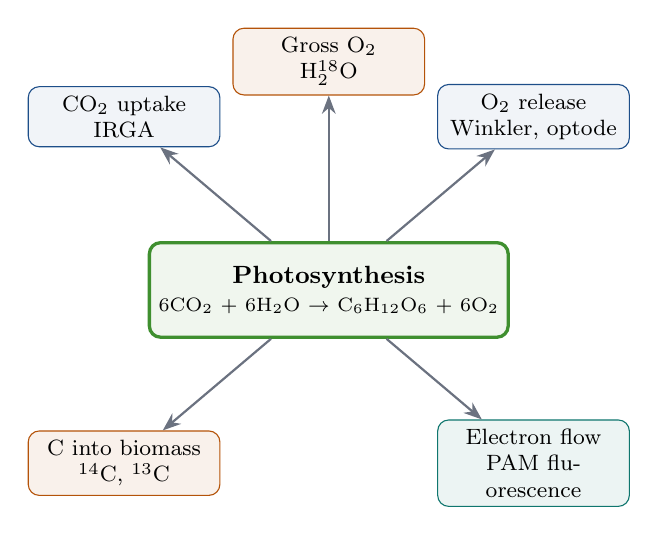
\begin{tikzpicture}[font=\small]
  \node[draw=leaf,very thick,rounded corners,fill=leaf!8,minimum width=4.2cm,minimum height=1.2cm,align=center] (ps) at (0,0) {\textbf{Photosynthesis}\\[-1pt]\scriptsize 6CO$_2$ + 6H$_2$O $\rightarrow$ C$_6$H$_{12}$O$_6$ + 6O$_2$};
  \node[draw=sea,rounded corners,fill=sea!6,align=center,text width=2.2cm,font=\footnotesize] (co2) at (-2.6,2.2) {CO$_2$ uptake\\IRGA};
  \node[draw=sea,rounded corners,fill=sea!6,align=center,text width=2.2cm,font=\footnotesize] (o2) at (2.6,2.2) {O$_2$ release\\Winkler, optode};
  \node[draw=warm,rounded corners,fill=warm!8,align=center,text width=2.2cm,font=\footnotesize] (c) at (-2.6,-2.2) {C into biomass\\$^{14}$C, $^{13}$C};
  \node[draw=accent,rounded corners,fill=accent!8,align=center,text width=2.2cm,font=\footnotesize] (e) at (2.6,-2.2) {Electron flow\\PAM fluorescence};
  \node[draw=warm,rounded corners,fill=warm!8,align=center,text width=2.2cm,font=\footnotesize] (o18) at (0,2.9) {Gross O$_2$\\H$_2^{18}$O};
  \foreach \n in {co2,o2,c,e,o18} \draw[-{Stealth},thick,grey] (ps) -- (\n);
\end{tikzpicture}}
\end{frame}

% 2 ---------------------------------------------------------------------
\begin{frame}{Gross, net and respiration}
\twocol{
\begin{itemize}
  \item \textbf{Net (NP)}: measured in the light; photosynthesis minus respiration
  \item \textbf{Respiration (R)}: measured in darkness
  \item \textbf{Gross}: GP = NP + R (if R is the same in light and dark)
  \item \textbf{PQ} = O$_2$ released / CO$_2$ fixed, about 1.0--1.4
  \item Normalise: per area, g mass, chlorophyll $a$ or m$^3$ water
\end{itemize}}{
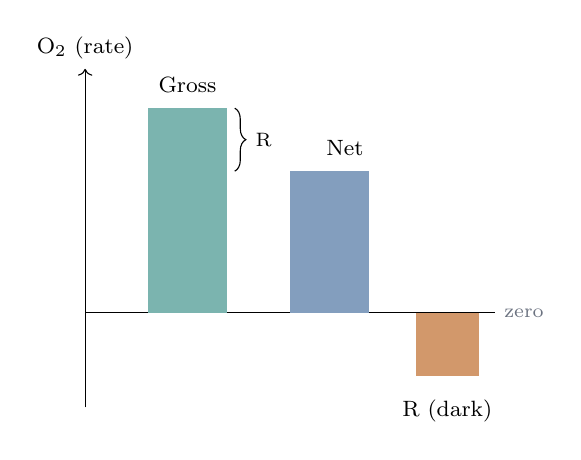
\begin{tikzpicture}[font=\small]
  \draw[->] (0,0) -- (0,4.3) node[above,font=\footnotesize] {O$_2$ (rate)};
  \draw (0,1.2) -- (5.2,1.2) node[right,font=\scriptsize,grey] {zero};
  \fill[accent!55] (0.8,1.2) rectangle (1.8,3.8); \node[font=\footnotesize,align=center] at (1.3,4.1) {Gross};
  \fill[sea!55] (2.6,1.2) rectangle (3.6,3.0); \node[font=\footnotesize] at (3.3,3.3) {Net};
  \fill[warm!60] (4.2,1.2) rectangle (5.0,0.4); \node[font=\footnotesize,align=center] at (4.6,-0.05) {R (dark)};
  \draw[decorate,decoration={brace,amplitude=4pt}] (1.9,3.8) -- (1.9,3.0) node[midway,right=4pt,font=\scriptsize] {R};
\end{tikzpicture}
\fignote{Schematic.}}
\end{frame}

% 3 ---------------------------------------------------------------------
\begin{frame}{Designing a P--I experiment}
\twocol{
\begin{itemize}
  \item A series of irradiances, from dark to saturating
  \item Each step: acclimate briefly, then measure the rate
  \item Hold temperature, CO$_2$ (DIC), O$_2$ and water motion constant
  \item Include darkness (R) and controls (no organism)
  \item Independent replicates; record mass, area or chlorophyll
\end{itemize}}{
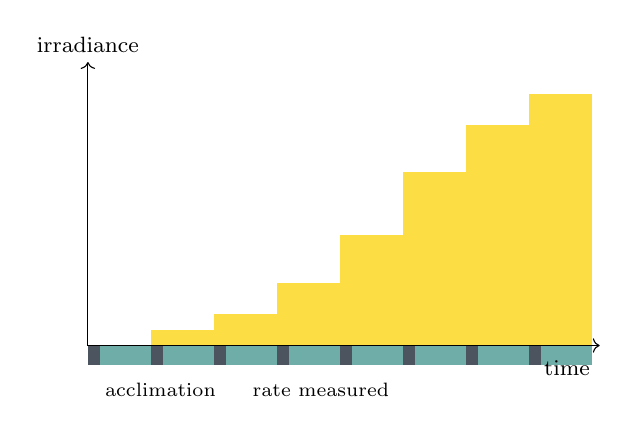
\begin{tikzpicture}[font=\small]
  \foreach \i/\h in {0/0,1/0.2,2/0.4,3/0.8,4/1.4,5/2.2,6/2.8,7/3.2}{
    \fill[yellow!70!orange,opacity=0.75] (\i*0.8,0) rectangle (\i*0.8+0.8,\h);
    \fill[ink!80] (\i*0.8,0) rectangle (\i*0.8+0.16,-0.25);
    \fill[accent!60] (\i*0.8+0.16,0) rectangle (\i*0.8+0.8,-0.25);}
  \draw[->] (0,0) -- (6.5,0) node[below left=2pt and 0pt,font=\footnotesize] {time};
  \draw[->] (0,0) -- (0,3.6) node[above,font=\footnotesize] {irradiance};
  \node[font=\scriptsize,anchor=north west] at (0,-0.35) {\textcolor{ink}{$\blacksquare$} acclimation \quad \textcolor{accent}{$\blacksquare$} rate measured};
\end{tikzpicture}
\fignote{Schematic of a stepped light series.}}
\end{frame}

% 4 ---------------------------------------------------------------------
\begin{frame}{Light and dark bottles (Winkler titration)}
\twocol{
\begin{itemize}
  \item Fill identical bottles with the same water (or algal suspension)
  \item Fix one immediately (initial), incubate one clear and one dark bottle
  \item Measure dissolved O$_2$ chemically (Winkler titration) at the end
  \item NP = (light $-$ initial)/$t$;\quad R = (initial $-$ dark)/$t$;\quad GP = NP + R
  \item Example (6 h): initial 7.80, light 8.45, dark 7.55 mg O$_2$ L$^{-1}$ gives GP = 0.150 mg O$_2$ L$^{-1}$ h$^{-1}$
\end{itemize}}{
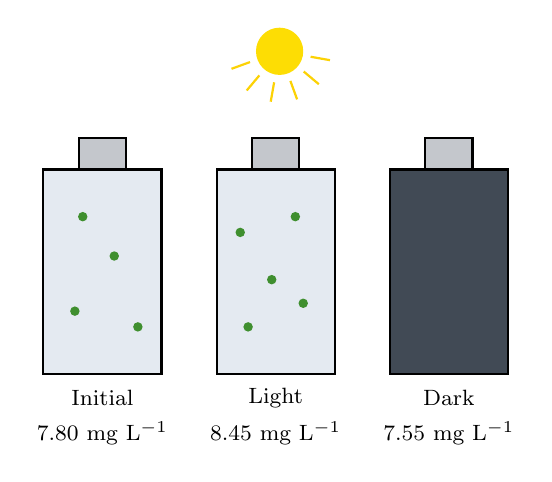
\begin{tikzpicture}[font=\small]
  \foreach \x/\lab/\fillc/\val in {0/Initial/sea!12/7.80,2.2/Light/sea!12/8.45,4.4/Dark/ink!85/7.55}{
    \draw[thick,fill=\fillc] (\x,0) rectangle (\x+1.5,2.6);
    \draw[thick,fill=grey!40] (\x+0.45,2.6) rectangle (\x+1.05,3.0);
    \node[font=\footnotesize] at (\x+0.75,-0.3) {\lab};
    \node[font=\footnotesize] at (\x+0.75,-0.75) {\val\ mg L$^{-1}$};}
  \foreach \p in {(2.6,0.6),(2.9,1.2),(3.3,0.9),(2.5,1.8),(3.2,2.0)} \fill[leaf] \p circle (0.06);
  \foreach \p in {(0.4,0.8),(0.9,1.5),(1.2,0.6),(0.5,2.0)} \fill[leaf] \p circle (0.06);
  \fill[yellow!80!orange] (3.0,4.1) circle (0.3);
  \foreach \a in {200,230,260,290,320,350} \draw[yellow!70!orange,thick] ($(3.0,4.1)+(\a:0.4)$) -- ($(3.0,4.1)+(\a:0.65)$);
\end{tikzpicture}}
\end{frame}

% 5 ---------------------------------------------------------------------
\begin{frame}{Oxygen sensors in a closed chamber}
\twocol{
\begin{itemize}
  \item Seaweed, seagrass, leaf discs or algae in a sealed chamber
  \item O$_2$ logged continuously: Clark electrode or optode
  \item Water jacket for temperature; stirrer thins the boundary layer
  \item Adjustable lamp; PAR measured at the sample
  \item Keep incubations short so O$_2$ and DIC change little
\end{itemize}}{
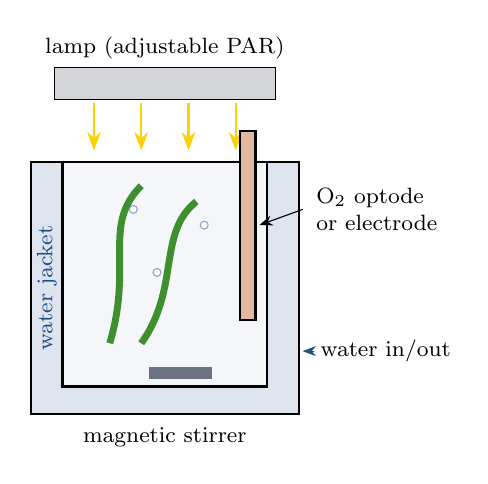
\begin{tikzpicture}[font=\footnotesize]
  % lamp
  \draw[fill=grey!30] (-0.4,4.0) rectangle (2.4,4.4); \node at (1.0,4.65) {lamp (adjustable PAR)};
  \foreach \x in {0.1,0.7,1.3,1.9} \draw[-{Stealth},yellow!70!orange,thick] (\x,3.95) -- (\x,3.35);
  % jacket and chamber
  \draw[thick,fill=sea!15] (-0.7,0) rectangle (2.7,3.2);
  \draw[thick,fill=sea!5] (-0.3,0.35) rectangle (2.3,3.2);
  \node[sea,rotate=90] at (-0.5,1.6) {water jacket};
  % seaweed
  \draw[leaf,line width=2.5pt] (0.3,0.9) .. controls (0.6,1.9) and (0.2,2.4) .. (0.7,2.9);
  \draw[leaf,line width=2.5pt] (0.7,0.9) .. controls (1.2,1.6) and (0.9,2.3) .. (1.4,2.7);
  \foreach \p in {(0.9,1.8),(1.5,2.4),(0.6,2.6)} \fill[white,draw=sea!50] \p circle (0.05);
  % stirrer
  \fill[grey] (0.8,0.45) rectangle (1.6,0.6); \node[anchor=north] at (1.0,-0.05) {magnetic stirrer};
  % sensor
  \draw[thick,fill=warm!40] (1.95,1.2) rectangle (2.15,3.6); \node[anchor=west,align=left] at (2.8,2.6) {O$_2$ optode\\or electrode};
  \draw[-{Stealth}] (2.75,2.6) -- (2.2,2.4);
  \draw[-{Stealth},sea] (2.9,0.8) -- (2.75,0.8) node[right=3pt,black] {water in/out};
\end{tikzpicture}
\fignote{Schematic, not to scale.}}
\end{frame}

% 6 ---------------------------------------------------------------------
\begin{frame}{From an oxygen trace to a rate}
\twocol{
\begin{itemize}
  \item Each light step gives a straight segment; its slope is the rate of O$_2$ change ($\mu$M min$^{-1}$)
  \item Discard the first minute (acclimation), fit a line to the rest
  \item Rate = slope $\times$ 60 $\times$ volume (L) / mass (g)
  \item Units: $\mu$mol O$_2$ g$^{-1}$ FW h$^{-1}$
  \item In darkness the slope is negative: respiration
\end{itemize}}{
\begin{tikzpicture}
\begin{axis}[height=5.8cm,xmin=0,xmax=40,xlabel={Time (min)},ylabel={O$_2$ ($\mu$mol L$^{-1}$)},
  tick label style={font=\footnotesize},label style={font=\small},xtick={0,5,...,40}]
  \foreach \x in {5,10,...,35} {\edef\temp{\noexpand\draw[grey!40] (axis cs:\x,230) -- (axis cs:\x,400);}\temp}
  \addplot[only marks,mark size=0.5pt,sea] table[x=t,y=c] {data/o2_trace.dat};
  \node[font=\scriptsize,anchor=south] at (axis cs:2.5,252) {0};
  \node[font=\scriptsize,anchor=south] at (axis cs:37.5,385) {800};
  \node[font=\scriptsize,grey,anchor=north west] at (axis cs:0.5,395) {PAR steps ($\mu$mol m$^{-2}$ s$^{-1}$)};
\end{axis}
\end{tikzpicture}
\fignote{Illustrative data: 2.0 g fresh mass of seaweed in 0.20 L, eight 5-min light steps (0--800 $\mu$mol m$^{-2}$ s$^{-1}$).}}
\end{frame}

% 7 ---------------------------------------------------------------------
\begin{frame}{The P--I curve and its parameters}
\twocol{
\begin{itemize}
  \item Plot rate against irradiance; fit $P = P_{max}\tanh(\alpha I/P_{max}) - R$
  \item $\alpha$: efficiency at low light; $P_{max}$: capacity
  \item $I_k = P_{max}/\alpha$: onset of saturation
  \item $I_c$: compensation point, where net rate = 0
  \item Example fit: $P_{max}$ = 30.0, $\alpha$ = 0.249, $R$ = 4.8; $I_k$ = 121, $I_c$ = 20
\end{itemize}}{
\begin{tikzpicture}
\begin{axis}[height=5.8cm,xmin=-20,xmax=840,ymin=-7,ymax=30,xlabel={PAR ($\mu$mol photons m$^{-2}$ s$^{-1}$)},
  ylabel={Net rate ($\mu$mol O$_2$ g$^{-1}$ h$^{-1}$)},tick label style={font=\footnotesize},label style={font=\small}]
  \addplot[grey!60] coordinates {(-20,0)(840,0)};
  \addplot[domain=0:820,samples=150,very thick,accent] {30.018*tanh(0.24875*x/30.018)-4.8396};
  \addplot[only marks,mark=*,mark size=2.2pt,sea] table[x=I,y=rate] {data/o2_rates.dat};
  \addplot[dashed,grey,domain=0:160] {0.24875*x-4.8396};
  \addplot[dashed,grey] coordinates {(120.7,-7)(120.7,30)};
  \node[font=\scriptsize,anchor=west] at (axis cs:125,-5) {$I_k$};
  \node[font=\scriptsize,anchor=south] at (axis cs:600,25.5) {$P_{max} - R$};
\end{axis}
\end{tikzpicture}
\fignote{Units: $P_{max}$ and $R$ in $\mu$mol O$_2$ g$^{-1}$ FW h$^{-1}$; $I_k$, $I_c$ in $\mu$mol photons m$^{-2}$ s$^{-1}$.}}
\end{frame}

% 8 ---------------------------------------------------------------------
\begin{frame}{Leaf gas exchange: the open system}
\twocol{
\begin{itemize}
  \item Air of known CO$_2$ flows through a clamp-on leaf chamber
  \item Infrared gas analysers (IRGAs) measure CO$_2$ (and H$_2$O) entering (reference) and leaving (sample)
  \item The leaf removes CO$_2$, so sample CO$_2$ is lower
  \item Chamber controls light, temperature, humidity and CO$_2$
  \item Also gives transpiration and stomatal conductance
\end{itemize}}{
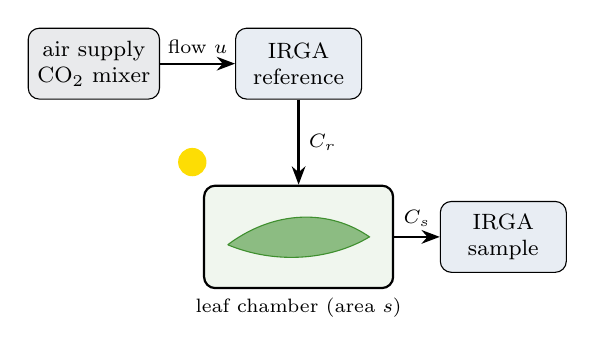
\begin{tikzpicture}[font=\footnotesize]
  \node[draw,fill=grey!15,rounded corners,align=center,minimum width=1.6cm,minimum height=0.9cm] (src) at (0,2.6) {air supply\\CO$_2$ mixer};
  \node[draw,fill=sea!10,rounded corners,align=center,minimum width=1.6cm,minimum height=0.9cm] (ref) at (2.6,2.6) {IRGA\\reference};
  \node[draw,thick,fill=leaf!8,rounded corners,minimum width=2.4cm,minimum height=1.3cm] (ch) at (2.6,0.4) {};
  \draw[leaf,fill=leaf!60] (1.7,0.3) .. controls (2.3,0.75) and (3.0,0.75) .. (3.5,0.4) .. controls (3.0,0.1) and (2.3,0.05) .. (1.7,0.3);
  \node[font=\scriptsize] at (2.6,-0.5) {leaf chamber (area $s$)};
  \node[draw,fill=sea!10,rounded corners,align=center,minimum width=1.6cm,minimum height=0.9cm] (smp) at (5.2,0.4) {IRGA\\sample};
  \draw[-{Stealth},thick] (src) -- node[above,font=\scriptsize]{flow $u$} (ref);
  \draw[-{Stealth},thick] (ref) -- node[right,font=\scriptsize]{$C_r$} (ch);
  \draw[-{Stealth},thick] (ch) -- node[above,font=\scriptsize]{$C_s$} (smp);
  \fill[yellow!80!orange] (1.25,1.35) circle (0.18);
\end{tikzpicture}
\fignote{Schematic of an open (flow-through) system.}}
\end{frame}

% 9 ---------------------------------------------------------------------
\begin{frame}{From CO$_2$ differences to a light response curve}
\twocol{
\begin{itemize}
  \item $A = u\,(C_r - C_s)/s$\quad (ignoring the small water-vapour correction)
  \item $u$ = 500 $\mu$mol s$^{-1}$, $s$ = 6 cm$^2$: a difference of 25 $\mu$mol mol$^{-1}$ means $A \approx$ 21 $\mu$mol CO$_2$ m$^{-2}$ s$^{-1}$
  \item Light steps usually run from high to low, with time to stabilise at each
  \item Same parameters as before: $A_{max}$, $\alpha$, $R_d$, $I_k$, $I_c$
\end{itemize}}{
\begin{tikzpicture}
\begin{axis}[height=5.8cm,xmin=-50,xmax=2100,ymin=-3,ymax=25,xlabel={PAR ($\mu$mol photons m$^{-2}$ s$^{-1}$)},
  ylabel={$A$ ($\mu$mol CO$_2$ m$^{-2}$ s$^{-1}$)},tick label style={font=\footnotesize},label style={font=\small}]
  \addplot[grey!60] coordinates {(-50,0)(2100,0)};
  \addplot[domain=0:2050,samples=200,very thick,leaf] {22.141*tanh(0.060397*x/22.141)-1.27};
  \addplot[only marks,mark=square*,mark size=2pt,ink] table[x=I,y=A] {data/irga.dat};
\end{axis}
\end{tikzpicture}
\fignote{Illustrative leaf: fit $A_{max}$ = 22.1, $\alpha$ = 0.060, $R_d$ = 1.27 $\mu$mol CO$_2$ m$^{-2}$ s$^{-1}$; $I_k$ = 367, $I_c$ = 21.}}
\end{frame}

% 10 --------------------------------------------------------------------
\begin{frame}{The $^{14}$C method}
\twocol{
\begin{itemize}
  \item Add a known amount of $^{14}$C-bicarbonate to light and dark bottles (Steemann Nielsen 1952)
  \item Incubate (often 2--24 h), filter, remove unfixed $^{14}$C with acid
  \item Count $^{14}$C fixed into organic matter (scintillation counter)
  \item Rate: {\small $P = \frac{DPM_{light} - DPM_{dark}}{DPM_{added}} \times \text{DIC} \times 1.05 / t$}
  \item Very sensitive: the standard for phytoplankton production
\end{itemize}}{
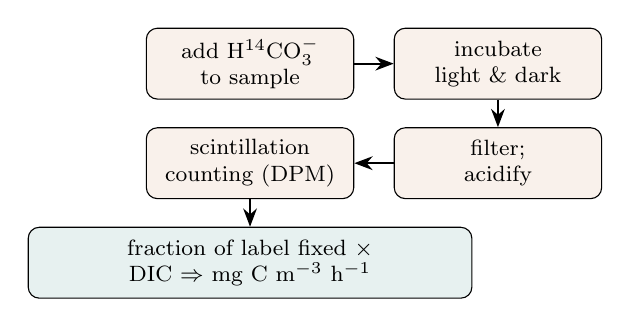
\begin{tikzpicture}[font=\footnotesize,node distance=0.35cm]
  \tikzset{st/.style={draw,rounded corners,fill=warm!8,align=center,text width=2.4cm,minimum height=0.9cm}}
  \node[st] (a) {add H$^{14}$CO$_3^-$\\to sample};
  \node[st,right=0.5cm of a] (b) {incubate\\light \& dark};
  \node[st,below=of b] (c) {filter;\\acidify};
  \node[st,left=0.5cm of c] (d) {scintillation\\counting (DPM)};
  \node[st,below=of d,fill=accent!10,text width=5.4cm] (e) {fraction of label fixed $\times$ DIC $\Rightarrow$ mg C m$^{-3}$ h$^{-1}$};
  \draw[-{Stealth},thick] (a) -- (b); \draw[-{Stealth},thick] (b) -- (c); \draw[-{Stealth},thick] (c) -- (d); \draw[-{Stealth},thick] (d) -- (e);
\end{tikzpicture}
\fignote{Example: 5 $\mu$Ci added, DIC 2.0 mmol L$^{-1}$, 2 h, light 3,350 and dark 150 DPM: $P$ = 3.6 mg C m$^{-3}$ h$^{-1}$.}}
\end{frame}

% 11 --------------------------------------------------------------------
\begin{frame}{Stable isotopes: $^{18}$O and $^{13}$C}
\twocol{
\begin{itemize}
  \item \textbf{H$_2^{18}$O}: add $^{18}$O-labelled water; O$_2$ from photosynthesis comes from water, so $^{18}$O$_2$ appears
  \item Measures \textbf{gross} O$_2$ production directly; respiration does not remove the label quickly
  \item \textbf{$^{13}$C}: non-radioactive alternative to $^{14}$C, measured by mass spectrometry
  \item Need mass spectrometers; more expensive, but no radioactive waste
\end{itemize}}{
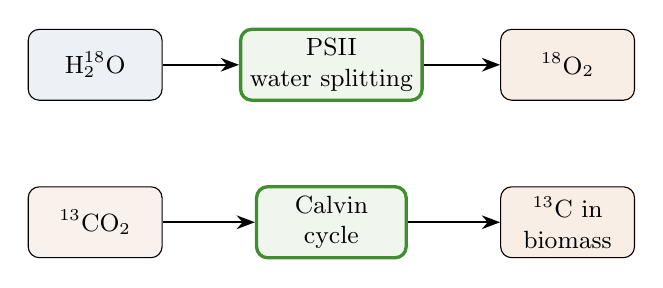
\begin{tikzpicture}[font=\small]
  \node[draw,rounded corners,fill=sea!8,minimum width=1.7cm,minimum height=0.9cm] (w) at (0,2) {H$_2^{18}$O};
  \node[draw=leaf,very thick,rounded corners,fill=leaf!8,minimum width=1.9cm,minimum height=0.9cm,align=center] (p) at (3,2) {PSII\\water splitting};
  \node[draw,rounded corners,fill=warm!10,minimum width=1.7cm,minimum height=0.9cm] (o) at (6,2) {$^{18}$O$_2$};
  \draw[-{Stealth},thick] (w) -- (p); \draw[-{Stealth},thick] (p) -- (o);
  \node[draw,rounded corners,fill=warm!8,minimum width=1.7cm,minimum height=0.9cm] (c) at (0,0) {$^{13}$CO$_2$};
  \node[draw=leaf,very thick,rounded corners,fill=leaf!8,minimum width=1.9cm,minimum height=0.9cm,align=center] (cc) at (3,0) {Calvin\\cycle};
  \node[draw,rounded corners,fill=warm!10,minimum width=1.7cm,minimum height=0.9cm,align=center] (b) at (6,0) {$^{13}$C in\\biomass};
  \draw[-{Stealth},thick] (c) -- (cc); \draw[-{Stealth},thick] (cc) -- (b);
\end{tikzpicture}}
\end{frame}

% 12 --------------------------------------------------------------------
\begin{frame}{Which rate does each method measure?}
\twocol{
\begin{itemize}
  \item $^{18}$O: gross O$_2$ production
  \item O$_2$ bottles: net (gross if light R = dark R)
  \item $^{14}$C: between gross and net, depending on incubation time (Peterson 1980)
  \item Fluorescence: electron transport, an upper limit to gross
  \item $^{14}$C often 60--100\% of $^{18}$O gross (Grande et al. 1989)
\end{itemize}}{
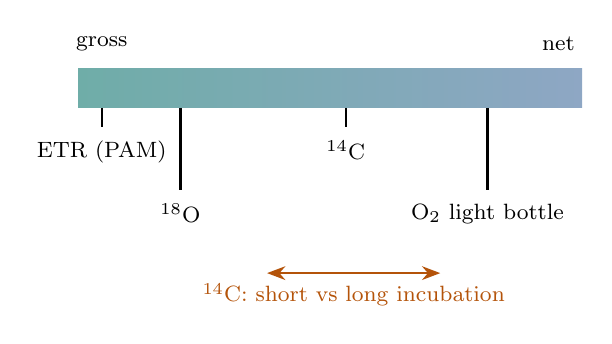
\begin{tikzpicture}[font=\footnotesize]
  \shade[left color=accent!60,right color=sea!50] (0,0) rectangle (6.4,0.5);
  \node[anchor=south] at (0.3,0.6) {gross}; \node[anchor=south] at (6.1,0.6) {net};
  \foreach \x/\lab/\y in {0.3/ETR (PAM)/-0.5,1.3/$^{18}$O/-1.3,3.4/$^{14}$C/-0.5,5.2/O$_2$ light bottle/-1.3}{
    \draw[thick] (\x,0) -- (\x,\y+0.25); \node[anchor=north,align=center] at (\x,\y+0.2) {\lab};}
  \draw[{Stealth}-{Stealth},thick,warm] (2.4,-2.1) -- (4.6,-2.1) node[midway,below] {$^{14}$C: short vs long incubation};
\end{tikzpicture}
\fignote{Schematic; positions are qualitative.}}
\end{frame}

% 13 --------------------------------------------------------------------
\begin{frame}{Chlorophyll fluorescence: three fates of absorbed light}
\twocol{
\begin{itemize}
  \item Light absorbed by PSII is used in photochemistry, lost as heat, or re-emitted as fluorescence
  \item The three compete: when photochemistry falls, fluorescence and heat rise
  \item Fluorescence can therefore report the efficiency of photochemistry
  \item PAM fluorometers use a modulated measuring light, so fluorescence can be measured even in sunlight
\end{itemize}}{
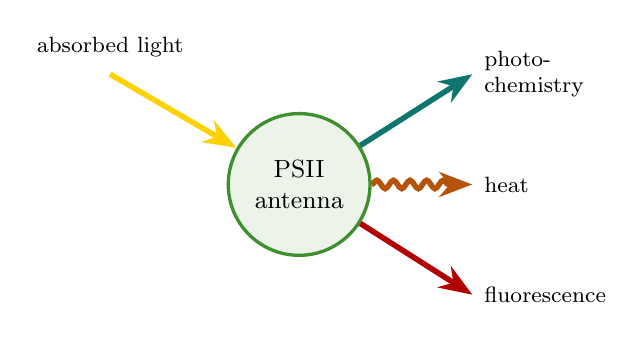
\begin{tikzpicture}[font=\small,xshift=-1cm]
  \node[draw=leaf,very thick,circle,fill=leaf!10,minimum size=1.8cm,align=center] (ch) at (0,0) {PSII\\antenna};
  \draw[-{Stealth},line width=2pt,yellow!70!orange] (-2.4,1.4) -- (ch); \node[font=\footnotesize,anchor=south] at (-2.4,1.5) {absorbed light};
  \draw[-{Stealth},line width=2pt,accent] (ch) -- (2.2,1.4) node[right,black,font=\footnotesize,align=left] {photo-\\chemistry};
  \draw[-{Stealth},line width=2pt,warm,decorate,decoration={snake,amplitude=1.5pt,segment length=6pt,post length=2mm}] (ch) -- (2.2,0) node[right,black,font=\footnotesize] {heat};
  \draw[-{Stealth},line width=2pt,red!70!black] (ch) -- (2.2,-1.4) node[right,black,font=\footnotesize] {fluorescence};
\end{tikzpicture}}
\end{frame}

% 14 --------------------------------------------------------------------
\begin{frame}{The saturating pulse}
\twocol{
\begin{itemize}
  \item Dark-adapted: $F_0$ (minimum), then a strong pulse closes all PSII centres: $F_m$
  \item $F_v/F_m = (F_m - F_0)/F_m$: maximum quantum yield (healthy leaves $\approx$ 0.8)
  \item In actinic light: steady $F$, and a pulse gives $F_m'$
  \item $\Phi_{PSII} = (F_m' - F)/F_m'$: effective quantum yield (Genty et al. 1989)
  \item Example: $F$ = 600, $F_m'$ = 950 gives $\Phi_{PSII}$ = 0.37
\end{itemize}}{
\begin{tikzpicture}
\begin{axis}[height=5.8cm,xmin=0,xmax=120,ymin=0,ymax=1850,xlabel={Time (s)},ylabel={Fluorescence (relative)},
  tick label style={font=\footnotesize},label style={font=\small}]
  \fill[yellow!30] (axis cs:30,0) rectangle (axis cs:120,1850);
  \addplot[very thick,red!70!black] table[x=t,y=F] {data/pam_trace.dat};
  \node[font=\scriptsize,anchor=north] at (axis cs:10,290) {$F_0$};
  \node[font=\scriptsize,anchor=south] at (axis cs:20.4,1510) {$F_m$};
  \node[font=\scriptsize,anchor=south] at (axis cs:60.4,960) {$F_m'$};
  \node[font=\scriptsize,anchor=north] at (axis cs:105,590) {$F$};
  \node[font=\scriptsize,anchor=north west] at (axis cs:31,1800) {actinic light on};
\end{axis}
\end{tikzpicture}
\fignote{Schematic trace (values chosen for illustration).}}
\end{frame}

% 15 --------------------------------------------------------------------
\begin{frame}{Electron transport rate and rapid light curves}
\twocol{
\begin{itemize}
  \item ETR = $\Phi_{PSII}$ $\times$ PAR $\times$ 0.5 $\times$ absorptance (0.84 for many leaves)
  \item Rapid light curve: short (e.g. 10 s) steps of increasing light, a pulse at each
  \item Fit the same tanh model: ETR$_{max}$, $\alpha$, $E_k$ (Ralph \& Gademann 2005)
  \item Fast and non-invasive: suits field work, seagrasses and seaweeds in situ
\end{itemize}}{
\begin{tikzpicture}
\begin{axis}[height=5.8cm,xmin=-20,xmax=1250,ymin=0,ymax=125,xlabel={PAR ($\mu$mol photons m$^{-2}$ s$^{-1}$)},
  ylabel={ETR ($\mu$mol e$^-$ m$^{-2}$ s$^{-1}$)},tick label style={font=\footnotesize},label style={font=\small}]
  \addplot[domain=0:1220,samples=150,very thick,accent] {110.62*tanh(0.33*x/110.62)};
  \addplot[only marks,mark=triangle*,mark size=2.6pt,red!70!black] table[x=I,y=ETR] {data/rlc.dat};
\end{axis}
\end{tikzpicture}
\fignote{Illustrative rapid light curve: ETR$_{max}$ = 111 $\mu$mol e$^-$ m$^{-2}$ s$^{-1}$, $\alpha$ = 0.33, $E_k$ = 334 $\mu$mol photons m$^{-2}$ s$^{-1}$.}}
\end{frame}

% 16 --------------------------------------------------------------------
\begin{frame}{Fluorescence: strengths and cautions}
\twocol{
\begin{itemize}
  \item Fast, no enclosure, works in situ (Diving-PAM)
  \item Counts electrons, not C or O$_2$: 4 e$^-$ per O$_2$ in theory
  \item Absorptance often assumed: \emph{relative} ETR
  \item Light history changes RLC parameters
  \item Calibrate against O$_2$ or $^{14}$C for absolute rates (Beer et al. 1998)
\end{itemize}}{
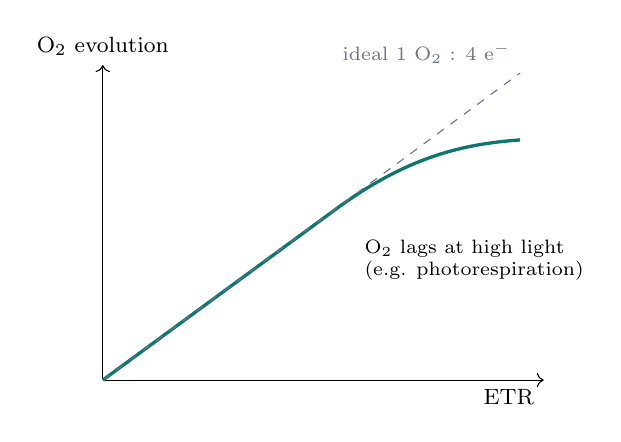
\begin{tikzpicture}[font=\small]
  \draw[->] (0,0) -- (5.6,0) node[below left,font=\footnotesize] {ETR};
  \draw[->] (0,0) -- (0,4) node[above,font=\footnotesize] {O$_2$ evolution};
  \draw[very thick,accent] (0,0) -- (3,2.2) .. controls (3.9,2.85) and (4.6,3.0) .. (5.3,3.05);
  \draw[dashed,grey] (0,0) -- (5.3,3.9);
  \node[font=\scriptsize,grey,anchor=south east] at (5.3,3.9) {ideal 1 O$_2$ : 4 e$^-$};
  \node[font=\scriptsize,align=left,anchor=north west] at (3.2,1.9) {O$_2$ lags at high light\\(e.g. photorespiration)};
\end{tikzpicture}
\fignote{Schematic, after the pattern described by Beer et al. (1998).}}
\end{frame}

% 17 --------------------------------------------------------------------
\begin{frame}{Seaweeds and seagrasses}
\twocol{
\begin{itemize}
  \item Usually O$_2$ evolution in stirred, temperature-controlled chambers
  \item Stirring matters: a thick boundary layer limits supply of CO$_2$/HCO$_3^-$
  \item In situ chambers enclose whole kelp or reef communities (Rodgers et al. 2015)
  \item Diving-PAM for in situ ETR and rapid light curves (Ralph et al. 1998)
  \item Normalise to fresh or dry mass, area or chlorophyll
\end{itemize}}{
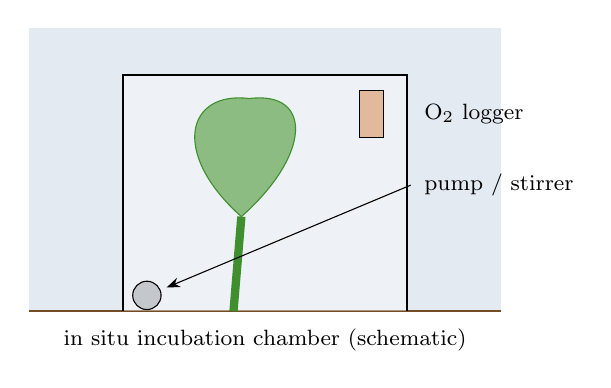
\begin{tikzpicture}[font=\footnotesize]
  \fill[sea!12] (0,0) rectangle (6,3.6);
  \draw[thick,brown!60!black] (0,0) -- (6,0);
  \draw[thick,fill=white,fill opacity=0.4] (1.2,0) -- (1.2,3.0) -- (4.8,3.0) -- (4.8,0);
  \draw[leaf,line width=3pt] (2.6,0) -- (2.7,1.2);
  \draw[leaf,fill=leaf!60] (2.7,1.2) .. controls (1.8,2.0) and (2.0,2.8) .. (2.8,2.7) .. controls (3.6,2.8) and (3.6,2.0) .. (2.7,1.2);
  \draw[fill=warm!40] (4.2,2.2) rectangle (4.5,2.8); \node[anchor=west] at (4.9,2.5) {O$_2$ logger};
  \draw[fill=grey!40] (1.5,0.2) circle (0.18); \node[anchor=west] at (4.9,1.6) {pump / stirrer};
  \draw[-{Stealth}] (4.85,1.6) -- (1.75,0.3);
  \node[anchor=north] at (3,-0.1) {in situ incubation chamber (schematic)};
\end{tikzpicture}}
\end{frame}

% 18 --------------------------------------------------------------------
\begin{frame}{Microalgae and phytoplankton}
\twocol{
\begin{itemize}
  \item Cells are dilute, so rates per bottle are small: sensitive methods are needed
  \item $^{14}$C incubations in a photosynthetron (many light levels at once) give P--I curves
  \item O$_2$ light--dark bottles and $^{18}$O for gross and net rates
  \item Normalise to chlorophyll $a$: $P^B_{max}$, $\alpha^B$
  \item Active fluorescence (PAM, FRRF) for high-frequency, in situ estimates
\end{itemize}}{
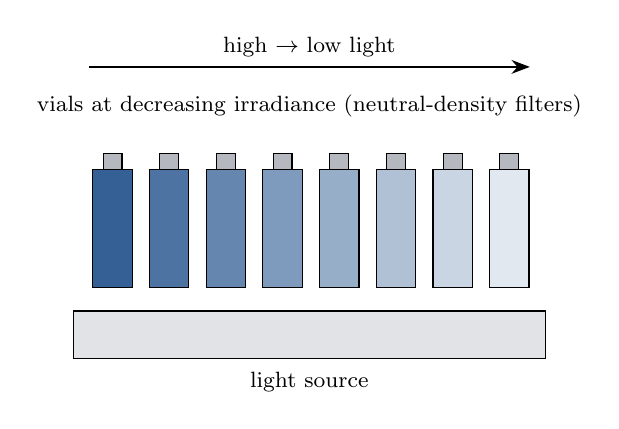
\begin{tikzpicture}[font=\footnotesize]
  \draw[fill=grey!20] (0,0) rectangle (6,0.6); \node at (3,-0.3) {light source};
  \foreach \i in {0,...,7}{
    \pgfmathsetmacro{\shade}{90-\i*11}
    \draw[fill=sea!\shade] (0.25+\i*0.72,0.9) rectangle (0.75+\i*0.72,2.4);
    \draw[fill=grey!50] (0.38+\i*0.72,2.4) rectangle (0.62+\i*0.72,2.6);}
  \node[align=center] at (3,3.2) {vials at decreasing irradiance (neutral-density filters)};
  \draw[-{Stealth},thick] (0.2,3.7) -- (5.8,3.7) node[midway,above] {high $\rightarrow$ low light};
\end{tikzpicture}
\fignote{Schematic photosynthetron.}}
\end{frame}

% 19 --------------------------------------------------------------------
\begin{frame}{Terrestrial plants: leaf to canopy}
\twocol{
\begin{itemize}
  \item Portable gas exchange: light and CO$_2$ responses of attached leaves (Long \& Bernacchi 2003)
  \item Leaf-disc O$_2$ electrodes: capacity at high CO$_2$
  \item Fluorescence: rapid stress screening ($F_v/F_m$)
  \item Canopies: large chambers or eddy covariance towers
  \item A leaf rate is not a canopy rate
\end{itemize}}{
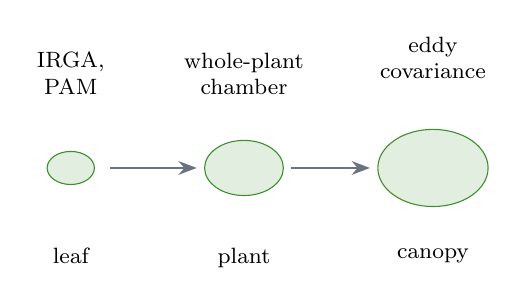
\begin{tikzpicture}[font=\footnotesize]
  \foreach \x/\s/\lab in {0/0.6/leaf,2.2/1.0/plant,4.6/1.4/canopy}{
    \node[draw=leaf,fill=leaf!15,ellipse,minimum width=\s cm,minimum height=\s cm*0.7] at (\x,1.2) {};
    \node[anchor=north] at (\x,0.3) {\lab};}
  \draw[-{Stealth},thick,grey] (0.5,1.2) -- (1.6,1.2); \draw[-{Stealth},thick,grey] (2.8,1.2) -- (3.8,1.2);
  \node[align=center] at (0,2.4) {IRGA,\\PAM}; \node[align=center] at (2.2,2.4) {whole-plant\\chamber}; \node[align=center] at (4.6,2.6) {eddy\\covariance};
\end{tikzpicture}}
\end{frame}

% 20 --------------------------------------------------------------------
\begin{frame}{Choosing a method}
\centering\footnotesize
\renewcommand{\arraystretch}{1.25}
\begin{tabular}{@{}>{\raggedright\arraybackslash}p{2.6cm}>{\raggedright\arraybackslash}p{2.7cm}>{\raggedright\arraybackslash}p{3.0cm}>{\raggedright\arraybackslash}p{4.5cm}@{}}
\toprule
\textbf{Method} & \textbf{Measures} & \textbf{Typical use} & \textbf{Main limitation}\\\midrule
Winkler bottles & net, gross (O$_2$) & plankton, lakes & slow; low sensitivity at low biomass\\
O$_2$ electrode/optode & net O$_2$ (continuous) & seaweeds, leaf discs, algae & enclosure; stirring and O$_2$ build-up\\
IRGA gas exchange & net CO$_2$ & leaves, whole plants & air only; chamber conditions\\
$^{14}$C & C fixed (gross--net) & phytoplankton & radioactive; meaning depends on incubation time\\
$^{18}$O / $^{13}$C & gross O$_2$ / C fixed & plankton, cultures & mass spectrometry; cost\\
PAM fluorescence & electron transport & everything, in situ & relative; not carbon fixation\\
\bottomrule
\end{tabular}
\end{frame}

% 21 --------------------------------------------------------------------
\begin{frame}{Summary}
\begin{itemize}
  \item Photosynthesis can be followed through CO$_2$, O$_2$, carbon or electrons; each method sees a different part
  \item Distinguish gross, net and respiration, and state how rates are normalised
  \item Good design: stepped irradiance, acclimation, constant conditions, controls, replicates
  \item Raw data (slopes, CO$_2$ differences, DPM, fluorescence yields) become rates by simple equations
  \item Rates against irradiance give P--I curves; fitted parameters ($\alpha$, $P_{max}$, $I_k$, $I_c$, $R$) let us compare species, sites and treatments
  \item Choose the method that matches the organism, the scale and the question
\end{itemize}
\end{frame}

\end{document}
